\documentclass[numbers=noenddot]{beamer}

\usepackage{tikz-cd}
\usepackage{sansmathfonts}
\usepackage{hhline}
\usepackage{subcaption}
\usetikzlibrary{automata,arrows.meta,positioning,patterns}
\renewcommand{\familydefault}{\sfdefault}
\DeclareFontSeriesDefault[sf]{bf}{bx}
\usepackage{pgfplots}
\usepgfplotslibrary{groupplots}

\usepackage{newunicodechar}
\newunicodechar{∀}{\ensuremath{\forall}}
\newunicodechar{∃}{\ensuremath{\exists}}
\newunicodechar{≤}{\ensuremath{\le}}
\newunicodechar{≰}{\ensuremath{\nleq}}
\newunicodechar{≡}{\ensuremath{\equiv}}
\newunicodechar{≥}{\ensuremath{\ge}}
\newunicodechar{∈}{\ensuremath{\in}}
\newunicodechar{∉}{\ensuremath{\notin}}
\newunicodechar{⊆}{\ensuremath{\subseteq}}
\newunicodechar{⊇}{\ensuremath{\supseteq}}
\newunicodechar{⊊}{\ensuremath{\subsetneq}}
\newunicodechar{⊈}{\ensuremath{\nsubseteq}}
\newunicodechar{⊗}{\ensuremath{\otimes}}
\newunicodechar{∧}{\ensuremath{\wedge}}
\newunicodechar{∨}{\ensuremath{\vee}}
\newunicodechar{Σ}{\ensuremath{\Sigma}}
\newunicodechar{≅}{\ensuremath{\cong}}
\newunicodechar{≠}{\ensuremath{\neq}}
\newunicodechar{∩}{\ensuremath{\cap}}
\newunicodechar{∪}{\ensuremath{\cup}}
\newunicodechar{δ}{\ensuremath{\delta}}
\newunicodechar{→}{\ensuremath{\to}}
\newunicodechar{τ}{\ensuremath{\tau}}
\newunicodechar{α}{\ensuremath{\alpha}}
\newunicodechar{β}{\ensuremath{\beta}}
\newunicodechar{γ}{\ensuremath{\gamma}}
\newunicodechar{μ}{\ensuremath{\mu}}
\newunicodechar{¬}{\ensuremath{\neg}}
\newunicodechar{λ}{\ensuremath{\lambda}}
\newunicodechar{ε}{\ensuremath{\varepsilon}}
\newunicodechar{ι}{\ensuremath{\iota}}
\newunicodechar{θ}{\ensuremath{\theta}}
\newunicodechar{×}{\ensuremath{\times}}
\newunicodechar{·}{\ensuremath{\cdot}}
\newunicodechar{∘}{\ensuremath{\circ}}
\newunicodechar{⟦}{\ensuremath{{\llbracket}}}
\newunicodechar{⟧}{\ensuremath{{\rrbracket}}}
\newunicodechar{⇔}{\ensuremath{{\ \Longleftrightarrow\ }}}
\newunicodechar{⇒}{\ensuremath{\implies}}
\newunicodechar{↦}{\ensuremath{\mapsto}}
\newunicodechar{⋀}{\ensuremath{\bigwedge}}
\newunicodechar{⋁}{\ensuremath{\bigvee}}
\newunicodechar{⋃}{\ensuremath{\bigcup}}
\newunicodechar{⊤}{\ensuremath{\top}}
\newunicodechar{⊥}{\ensuremath{\bot}}
\newunicodechar{∅}{\ensuremath{\emptyset}}

\newcommand{\JSL}{\textbf{JSL}}
\newcommand{\JSLf}{\ensuremath{\mathbf{JSL}_\mathbf{f}}}
\newcommand{\Dep}{\textbf{Dep}}
\newcommand{\Rel}{\textbf{Rel}}
\newcommand{\mH}{\ensuremath{\mathcal{H}}}
\newcommand{\mG}{\ensuremath{\mathcal{G}}}
\newcommand{\mR}{\ensuremath{\mathcal{R}}}
\newcommand{\mP}{\ensuremath{\mathcal{P}}}
\newcommand{\mT}{\ensuremath{\mathcal{T}}}
\newcommand{\mS}{\ensuremath{\mathcal{S}}}
\newcommand{\mQ}{\ensuremath{\mathcal{Q}}}
\newcommand{\dr}{\ensuremath{\text{dr}}}
\newcommand{\DR}{\ensuremath{\mathcal{DR}}}
\newcommand{\GD}{\ensuremath{\mathcal{GD}}}
\newcommand{\SP}{\ensuremath{\mathcal{SP}}}
\newcommand{\SD}{\ensuremath{\mathcal{SD}}}
\newcommand{\LD}{\ensuremath{\text{LD}}}
\newcommand{\SLD}{\ensuremath{\text{SLD}}}
\newcommand{\BLD}{\ensuremath{\text{BLD}}}
\newcommand{\BLRD}{\ensuremath{\text{BLRD}}}
\newcommand{\op}{\ensuremath{\text{op}}}
\newcommand{\dfa}{\ensuremath{\textbf{dfa}}}
\newcommand{\natm}{\ensuremath{\textbf{natm}}}
\newcommand{\nsyn}{\ensuremath{\textbf{nsyn}}}
\newcommand{\ns}{\ensuremath{\textbf{ns}}}
\newcommand{\syn}{\ensuremath{\textrm{syn}}}
\newcommand{\synL}{{\syn(L)}}
\newcommand{\synLr}{{\syn(L^r)}}
\newcommand{\langs}{\ensuremath{\textrm{langs}}}
\newcommand{\rsc}{\ensuremath{\textrm{rsc}}}
\newcommand{\PSPACE}{\textsc{PSPACE}}
\newcommand{\NP}{\textsc{NP}}

\newcommand{\since}{\ensuremath{\text{since\ }}}
\newcommand{\definedAs}{\ensuremath{:\Leftrightarrow}}
\newcommand{\nerEq}{{\thicksim_L}}
\newcommand{\nerEqR}{{\thicksim_{L^r}}}
\newcommand{\sEq}{{≡_L}}
\newcommand{\sEqR}{{≡_{L^r}}}

\newlength{\leftstackrelawd}
\newlength{\leftstackrelbwd}
\def\leftstackrel#1#2{\settowidth{\leftstackrelawd}%
{${{}^{#1}}$}\settowidth{\leftstackrelbwd}{$#2$}%
\addtolength{\leftstackrelawd}{-\leftstackrelbwd}%
\leavevmode\ifthenelse{\lengthtest{\leftstackrelawd>0pt}}%
{\kern-.5\leftstackrelawd}{}\mathrel{\mathop{#2}\limits^{#1}}}


\title{Syntactic NFA Minimization via SAT solving}
\author{Bastian Kauschke}
\date{\today}
\logo{
\includegraphics[height=0.7cm,trim=0cm -5mm 0 0mm]{img/fau}}

\addtobeamertemplate{navigation symbols}{}{%
    \usebeamerfont{footline}%
    \usebeamercolor[fg]{footline}%
    \hspace{1em}%
    \insertframenumber
}

\begin{document}
\begin{frame}
\begin{center}
    \titlepage
\end{center}
\end{frame}

\begin{frame}
\begin{center}
    \large{GOAL}

    \vspace{1cm}

    minimal nfas
\end{center}
\end{frame}

\begin{frame}
   Given an nfa $M$ with states $Q$, nfa $N$ with states $S$ is a \textit{union nfa} of $M$ if
    \begin{itemize}
        \item each $s ∈ S$ accepts $⋃\{ L(N, q) : q ∈ X \}$ with $X ⊆ Q$
        \item $L(N) = L(M)$
    \end{itemize}
    \pause
    \vspace{1cm}
    An nfa $N$ is \textit{rpd} if $N^R$ is a partial dfa.

    The states of rpd nfas accept pairwise disjoint languages.

    All trimmed nfas whose states accept pairwise disjoint languages are rpd.
\end{frame}

\begin{frame}
    nfa $N = (Q, δ, I, F)$ accepting $L$ is \textbf{atomic} if the following equivalent statements hold
    \begin{itemize}
        \item $\rsc(N^R)$ is a minimal dfa
        \item each $q ∈ Q$ accepts a language from $\BLD(L)$, the closure of $\LD(L)$ under all set-theoretic boolean operations
        \item each $q ∈ Q$ accepts a union of congruence classes of the \textit{Nerode left congruence} $\nerEq$:
        \begin{align*}
            u \nerEq v &⇔ ∀x ∈ Σ^*. u ∈ x^{-1}L = v ∈ x^{-1}L\\
                       &⇔ (u^r)^{-1}L^r = (v^r)^{-1}L^r
        \end{align*}
        \item[\textcolor{red}{$\blacktriangleright$}] $N$ is a union nfa of the átomaton $\dfa(L^r)^R$
    \end{itemize}
\end{frame}

\begin{frame}
    nfa $N = (Q, δ, I, F)$ accepting $L$ is \textbf{subatomic} if the following equivalent statements hold
    \begin{itemize}
        \item the transition monoid of $\rsc(N^R)$ is isomorphic to $\synLr$
        \item each $q ∈ Q$ accepts a language from $\BLRD(L)$, the closure of $\LD(L)$ under all boolean operations and right derivatives
        \item each $q ∈ Q$ accepts a union of congruence classes of the \textit{syntactic congruence} $\sEq$:
        \begin{align*}
            u \sEq v &⇔ ∀x, y ∈Σ^*. u ∈ x^{-1}Ly^{-1} = v ∈ x^{-1}Ly^{-1}
        \end{align*}
        \item[\textcolor{red}{$\blacktriangleright$}] $N$ is a union nfa of the syntactic nfa $\mathbf{syn}(L)$
    \end{itemize}
\end{frame}

\begin{frame}
    \begin{center}
        given $\dfa(L)$ and an rpd nfa $M = (Q, δ, I, \{ q_f \})$ accepting $L$,

        \vspace{1cm}

        does a union nfa $N$ of $M$ with $k$ states exist?
    \end{center}
\end{frame}

\begin{frame}[fragile]
    We are searching for an nfa $N$ with states $\mathbf{k}$:
    \begin{itemize}
        \pause
        \item $N$ is a union nfa: $H ⊆ \mathbf{k} × Q$
        $$H[i] = X ⇔ L(N, i) = ⋃\{ L(M, q) : q ∈ X \}$$
        \pause
        \item $N$ accepts $L$: $G ⊆ \LD(L) × \mathbf{k}$
        $$G[u^{-1}L] = Y ⇔ u^{-1}L = ⋃\{ L(N, i) : i ∈ Y \}$$
    \end{itemize}
    
    \pause
    As a commutative diagram:
    \[\begin{tikzcd}
		{\LD(L)} &\\
		\mathbf{k} & Q
		\arrow["⊇", from=1-1, to=2-2]
		\arrow["G"', from=1-1, to=2-1]
		\arrow["H"', from=2-1, to=2-2]
	\end{tikzcd}\]
\end{frame}

\begin{frame}[fragile]
    Require states to accept their assigned language using the transition relations $R_a ⊆ \mathbf{k} ×  \mathbf{k}$ $(a ∈ Σ)$:

    \[\begin{tikzcd}
        \LD(L) & & & Q & Q\\
        \mathbf{k} & Q   & & \mathbf{k} & \mathbf{k}\\
        \arrow["G"', from=1-1, to=2-1]
        \arrow["⊇", from=1-1, to=2-2]
        \arrow["H"', from=2-1, to=2-2]
        \arrow["H", from=2-4, to=1-4]
        \arrow["H"', from=2-5, to=1-5]
        \arrow["δ_a", from=1-4, to=1-5]
        \arrow["R_a"', from=2-4, to=2-5]
    \end{tikzcd}\]
    \pause
    $$N = (\mathbf{k}, (R_a)_{a ∈ Σ}, G[L], H^{-1}[q_f])$$
\end{frame}

\begin{frame}[fragile]
    $$
        L = \{ w ∈ Σ^* : |w|_b = 0 ∨ |w|_a ≠ 1 \}
    $$


    \begin{center}
        
    \begin{figure}
      \begin{subfigure}{0.4\framewidth}
      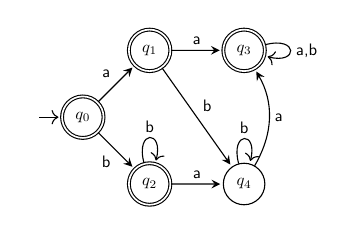
\begin{tikzpicture}[shorten >=1pt,node distance=1.2cm,on grid,auto,scale=0.6, every node/.style={scale=0.6}]
        \node[state,initial,accepting, initial text={},] (q_0) {$q_0$}; 
        \node[state,accepting] (q_1) [above right=of q_0] {$q_1$}; 
        \node[state,accepting] (q_2) [below right=of q_0] {$q_2$};
        \node[state,accepting] (q_3) [right=of q_1] {$q_3$}; 
        \node[state] (q_4) [right=of q_2] {$q_4$};
         \path[-stealth] 
         (q_0) 	edge  node {a} (q_1)
               edge  node [swap] {b} (q_2)
         (q_1) 	edge  node {a} (q_3)
                edge  node {b} (q_4)
         (q_2) 	edge  node {a} (q_4)
                edge [loop above] node {b}()
           (q_3) 	edge [loop right] node {a,b}()
         (q_4) 	edge [bend right] node [swap]{a} (q_3)
                edge [loop above] node {b}();
      \end{tikzpicture}
      \caption*{$\mathbf{dfa}(L)$}
      \end{subfigure}
      \begin{subfigure}{0.4\framewidth}
      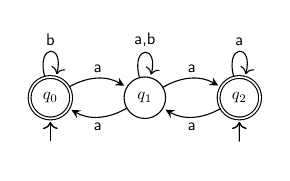
\begin{tikzpicture}[shorten >=1pt,node distance=1.2cm,on grid,auto,scale=0.6, every node/.style={scale=0.6}]
        \node[state,initial,accepting, initial text={}, initial below] (q_0) {$q_0$};
        \node[state] (q_1) [right=of q_0]{$q_1$};
        \node[state,initial,accepting, initial text={}, initial below] (q_2) [right=of q_1] {$q_2$};
         \path[-stealth] 
         (q_0) 	edge [bend left] node {a} (q_1)
                edge [loop above] node {b}()
         (q_1)	edge [bend left] node {a} (q_0)
             edge [bend left] node {a} (q_2)
            edge [loop above] node {a,b}()
         (q_2) 	edge [bend left] node {a} (q_1)
            edge [loop above] node {a}();
      \end{tikzpicture}
      \caption*{$N$}
      \end{subfigure}
      \end{figure}
    
      \begin{figure}
      \begin{subfigure}{0.4\framewidth}
      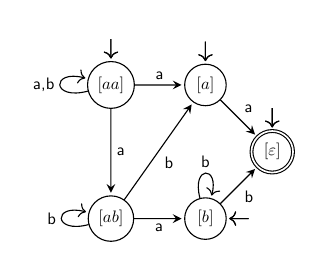
\begin{tikzpicture}[shorten >=1pt,node distance=1.2cm,on grid,auto,scale=0.6, every node/.style={scale=0.6}]
        \node[state,initial,accepting, initial text={}, initial above] (q_0) {$[\varepsilon]$}; 
        \node[state,initial, initial text={}, initial above] (q_1) [above left=of q_0] {$[\text{a}]$}; 
        \node[state,initial, initial text={}, initial right] (q_2) [below left=of q_0] {$[\text{b}]$};
        \node[state,initial, initial text={}, initial above] (q_3) [left=of q_1] {$[\text{aa}]$}; 
        \node[state] (q_4) [left=of q_2] {$[\text{ab}]$};
         \path[-stealth]
         (q_1) 	edge  node {a} (q_0)
         (q_2) 	edge  node [swap] {b} (q_0)
                edge [loop above] node {b}()
           (q_3) 	edge [loop left] node {a,b}()
             edge node {a} (q_1)
            edge node {a} (q_4)
         (q_4) 	edge node [swap] {b} (q_1)
              edge node [swap] {a} (q_2)
                edge [loop left] node {b}();
      \end{tikzpicture}
      \caption*{$\mathbf{syn}(L)$}
      \end{subfigure}
      \begin{subfigure}{0.4\framewidth}
      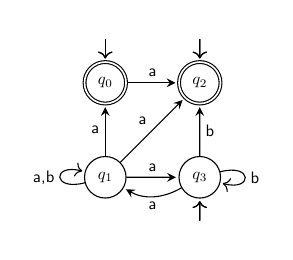
\begin{tikzpicture}[shorten >=1pt,node distance=1.2cm,on grid,auto,scale=0.6, every node/.style={scale=0.6}]
        \node[state,initial,accepting, initial text={}, initial above] (q_0) {$q_0$}; 
        \node[state] (q_1) [below=of q_0] {$q_1$}; 
        \node[state,initial,accepting, initial text={}, initial above] (q_2) [right=of q_0] {$q_2$};
        \node[state,initial, initial text={}, initial below] (q_3) [below=of q_2] {$q_3$};
         \path[-stealth]
         (q_0)  edge node {a} (q_2)
         (q_1) 	edge  node {a} (q_0)
             edge node {a} (q_2)
            edge node {a} (q_3)
            edge [loop left] node {a,b}()
           (q_3) 	edge [loop right] node {b}()
             edge node [swap] {b} (q_2)
             edge [bend left] node {a} (q_1);
      \end{tikzpicture}
      \caption*{$N_\mathds{syn}$}
      \end{subfigure}
      \end{figure}
    \end{center}
\end{frame}

\begin{frame}
    \frametitle{performance results}
    \begin{figure}[b]
        \centering
        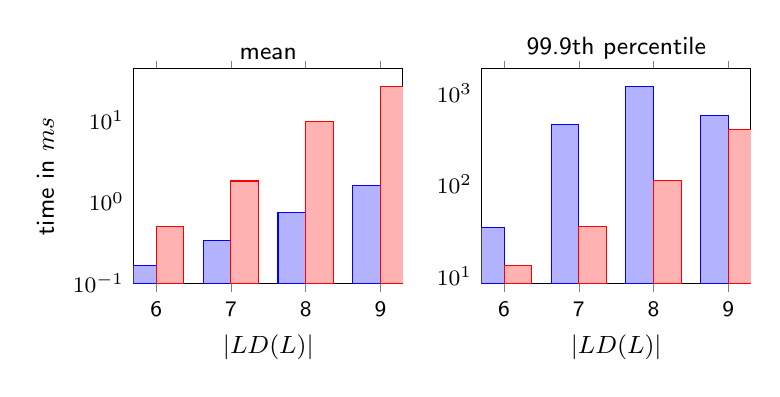
\begin{tikzpicture}
    \begin{groupplot}[
            legend columns=-1,
            footnotesize,
            ymode=log,
            ytick style={draw=none},
            ybar=0,
            % area legend, % This is the alternate option
            group style={
                group size=3 by 1,
                xlabels at=edge bottom,
                ylabels at=edge left,
            }
    ]
    \nextgroupplot[
        title={mean},
        ylabel={time in $ms$},
        xtick=data,
        xlabel={$|\LD(L)|$},
        symbolic x coords={6, 7, 8, 9},
        log origin=infty,
    ]
        \addplot coordinates {(6,0.162777) (7,0.334115) (8,0.729992) (9,1.583728)};
        \addplot coordinates {(6,0.490672) (7,1.784444) (8,9.631891) (9,25.491817)};
    
    \nextgroupplot[
        title={99.9th percentile},
        xtick=data,
        xlabel={$|\LD(L)|$},
        symbolic x coords={6, 7, 8, 9},
        log origin=infty,
    ]
        \addplot coordinates {(6,33.519221) (7,449.601883) (8,1164.183806) (9,564.966471)};
        \addplot coordinates {(6,12.812953) (7,34.571611) (8,110.581605) (9,395.503259)};
    
            \end{groupplot}
        \end{tikzpicture}
    \end{figure}
\end{frame}

\begin{frame}
    \frametitle{performance results}
    \begin{figure}
        \centering
        \begin{tikzpicture}
    \begin{groupplot}[
        legend columns=-1,
        footnotesize,
        ymode=log,
        ytick style={draw=none},
        ybar=0,
        ymax=25,
        ymin = 0.25,
        xtick distance = 50,
        xmin = 0,
        xmax = 300,
        % area legend, % This is the alternate option
        group style={
            group size=2 by 1,
            ylabels at=edge left,
        }
                    ]
                    \nextgroupplot[
                        title={\scriptsize \textbf{kw}, $|\LD(L)| = 8$},
                        ylabel={time in $ms$},
                        xlabel={$|\LD(L^r)|$},
                        width = \textwidth * 0.5,
                    ]
                    \addplot[only marks,mark=o] table[col sep=comma] {8dfa_lr_mean_kw.csv};
                    
                    \nextgroupplot[
                        title={\scriptsize \textbf{union}, $|\LD(L)| = 8$},
                        xlabel={$|\LD(L^r)|$},
                        width = \textwidth * 0.5,
                    ]
                    \addplot[only marks,mark=o] table[col sep=comma] {8dfa_lr_mean_atm.csv};
    \end{groupplot}
        \end{tikzpicture}
    \end{figure}
\end{frame}

\begin{frame}[fragile]
    \frametitle{size results}
    \resizebox{\framewidth}{!}{\begin{tabular}{ |c||c|c|c|c|c| }
		\hline
		k & total  & $\ns(L) < |\LD(L)|$ &  $\ns(L) < \natm(L)$ & $\ns(L) < \nsyn(L)$ & unknown \\
		\hhline{|=#=|=|=|=|=|}
        1  & \textbf{2} & \textbf{1} (50.0\%) & \textbf{0} (0.0\%) & \textbf{0} (0.0\%) & 0 \\
		\hline
        2  & \textbf{24} & \textbf{3} (12.5\%)&  \textbf{0} (0.0\%) & \textbf{0} (0.0\%) & 0 \\
		\hline
        3  & \textbf{1028} & \textbf{123} (12.0\%) &  \textbf{0} (0.0\%) & \textbf{0} (0.0\%) & 0 \\
		\hline
        4  & \textbf{56014} & \textbf{5911} (10.6\%) &  \textbf{86} (0.15\%) &\textbf{86} (0.15\%) & 0 \\
		\hline
        5 & \textbf{3705306} & \textbf{335820} (9.1\%)&  \textbf{13376} (0.36\%) & \textbf{11122} (0.30\%) & 0 \\
		\hline
        6 & 1269000 & 98376 (7.8\%) & 5399 (0.43\%) & 4540 (0.36\%) & 0 \\
		\hline
        7 & 1000000 & 67904 (6.8\%) & 4159 (0.42\%) & & 93 \\
        \hline
        8 & 1000000 & 60497 (6.0\%) & 4084 (0.41\%) & & 362 \\
        \hline
        9 & 1000000 & 55131 (5.5\%) & 3668 (0.37\%) & & 372 \\
        \hline
        10 & 1000000 & 51563 (5.2\%) & 3598 (0.36\%) & & 318 \\
        \hline
        11 & 1000000 & 48070 (4.8\%) & 3465 (0.34\%) & & 241 \\
        \hline
	\end{tabular}}
\end{frame}

\end{document}
